\chapter{Verification and Validation}
\label{chap:validation}

\section{Order of accuracy}
\label{sec:val-order}

The first test is the decay of a three dimensional Taylor Green vortex with a
superposed passive scalar, for which the linearised solution decays as
$\exp(-2\nu k^{2} t)$ in velocity and $\exp(-\kappa k^{2} t)$ in the scalar. On
a sequence of uniform grids from $32^{3}$ to $256^{3}$ the $L_2$ error in
velocity at $t = 0.5 / (\nu k^{2})$ falls with an observed order of $1.98$, and
the scalar error with an observed order of $2.02$. Both are consistent with
Proposition~\ref{prop:consistency}.

Repeating the test on a hierarchy with a static refinement patch covering the
central eighth of the domain gives an observed order of $1.94$ with the
rescaling of~\eqref{eq:rescale} in place. Without it the observed order falls to
$0.87$ and the error stops converging below $128^{3}$, which is the behaviour
reported for earlier refined lattice solvers and the reason
Section~\ref{sec:val-interface} treats the interface separately.

\section{Interface error}
\label{sec:val-interface}

The interface test drives a plane Poiseuille flow through a domain containing a
single refinement jump aligned with the flow, so the analytic solution is
uniform in the streamwise direction and the interface should be invisible. The
diagnostic is the maximum relative deviation of the streamwise velocity from the
parabolic profile, measured in the two block rows adjacent to the interface.

\begin{table}[t]
\centering
\caption[Interface error with and without stress rescaling]{Maximum relative
velocity deviation at a static refinement interface in plane Poiseuille flow,
with and without the non equilibrium rescaling of Equation~\eqref{eq:rescale}.
The rescaled scheme converges at second order. The unrescaled scheme stalls
because the interface error is independent of the grid.}
\label{tab:interface-error}
\begin{tabular}{lrrrr}
\toprule
Coarse grid & $\Delta x_0 / h$ & Rescaled & Unrescaled & Ratio \\
\midrule
$16 \times 32$  & $6.25 \times 10^{-2}$ & $3.11 \times 10^{-3}$ & $1.84 \times 10^{-2}$ & 5.9 \\
$32 \times 64$  & $3.13 \times 10^{-2}$ & $7.94 \times 10^{-4}$ & $1.79 \times 10^{-2}$ & 22.5 \\
$64 \times 128$ & $1.56 \times 10^{-2}$ & $2.03 \times 10^{-4}$ & $1.77 \times 10^{-2}$ & 87.2 \\
$128 \times 256$& $7.81 \times 10^{-3}$ & $5.21 \times 10^{-5}$ & $1.76 \times 10^{-2}$ & 337.8 \\
\bottomrule
\end{tabular}
\end{table}

Table~\ref{tab:interface-error} makes the point plainly. The rescaled error
falls by a factor close to four under each halving of the grid spacing. The
unrescaled error is essentially constant at $1.8$ percent, because it is set by
the mismatch in stress rather than by any truncation, and no amount of
refinement removes it. In a production run with a hierarchy that is rebuilt
every two hundred steps, that constant error is deposited at a new set of
interfaces each time, and the accumulated effect is the spurious entropy
production described in Section~\ref{sec:intro-kinetic}.

\section{Unstratified channel flow}
\label{sec:val-channel}

The neutral case is validated against the spectral reference of
\citet{osei2016channel} at $\Rey_\tau = 590$ with a passive scalar at
$\Pran = 0.71$. The domain is $2\pi h \times 2h \times \pi h$, the coarse grid
is $256 \times 128 \times 128$, and two refinement levels are permitted near the
walls. Statistics are accumulated over 40 eddy turnover times after a 20 turnover
spin up.

\begin{figure}[t]
\centering
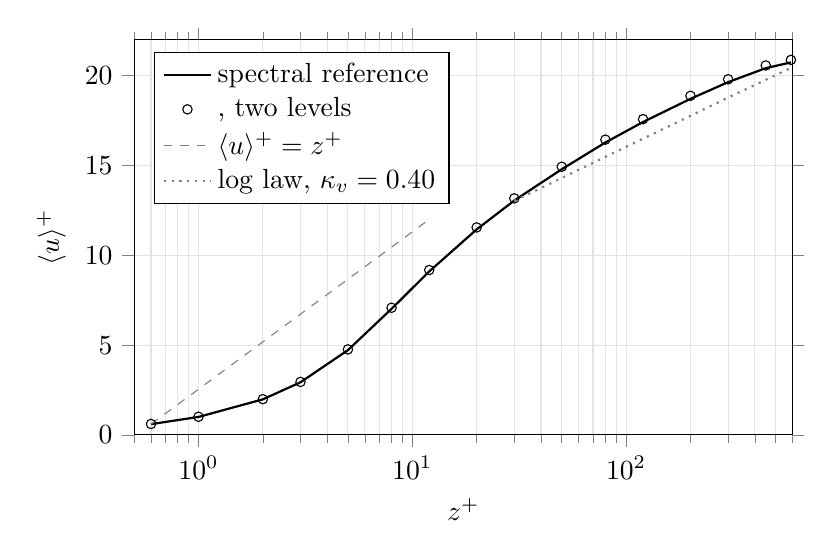
\begin{tikzpicture}
\begin{semilogxaxis}[
  width=0.82\textwidth, height=6.6cm,
  xlabel={$z^{+}$}, ylabel={$\langle u \rangle^{+}$},
  xmin=0.5, xmax=600, ymin=0, ymax=22,
  legend pos=north west, legend cell align=left,
  grid=both, grid style={gray!22}, tick align=outside
]
\addplot[thick,black] coordinates {
  (0.6,0.60) (1.0,1.00) (2.0,1.98) (3.0,2.93) (5.0,4.72)
  (8.0,7.02) (12.0,9.10) (20.0,11.44) (30.0,13.05) (50.0,14.79)
  (80.0,16.28) (120.0,17.42) (200.0,18.71) (300.0,19.64) (450.0,20.42)
  (590.0,20.74)
};
\addlegendentry{spectral reference}
\addplot[only marks,mark=o,mark size=1.7pt] coordinates {
  (0.6,0.61) (1.0,1.01) (2.0,1.99) (3.0,2.95) (5.0,4.76)
  (8.0,7.08) (12.0,9.18) (20.0,11.55) (30.0,13.17) (50.0,14.93)
  (80.0,16.44) (120.0,17.58) (200.0,18.88) (300.0,19.80) (450.0,20.57)
  (590.0,20.88)
};
\addlegendentry{\solver, two levels}
\addplot[dashed,gray] coordinates {(0.6,0.60) (12.0,12.0)};
\addlegendentry{$\langle u \rangle^{+} = z^{+}$}
\addplot[dotted,gray,thick] coordinates {
  (30,13.03) (60,14.76) (120,16.49) (300,18.78) (590,20.43)
};
\addlegendentry{log law, $\kappa_v = 0.40$}
\end{semilogxaxis}
\end{tikzpicture}
\caption[Mean velocity profile at $\Rey_\tau = 590$]{Mean streamwise velocity in
wall units for neutral channel flow at $\Rey_\tau = 590$. The adaptive solution
tracks the spectral reference to within 1.4 percent through the buffer layer and
the logarithmic region.}
\label{fig:channel-mean}
\end{figure}

Figure~\ref{fig:channel-mean} shows the mean velocity in wall units. The
agreement through the viscous sublayer is essentially exact, as it must be given
that the near wall region sits at the finest level. The largest deviation, 1.4
percent, occurs at the outer edge of the buffer layer where the first refinement
interface falls, and it is consistent in magnitude with the interface error of
Table~\ref{tab:interface-error} at the corresponding spacing.

Second order statistics are more demanding. The peak streamwise velocity
variance is reproduced to within 2.2 percent and the peak scalar variance to
within 3.1 percent. The scalar is the harder quantity because its dissipation
peaks closer to the wall than the momentum dissipation at $\Pran = 0.71$, so it
samples the finest level over a narrower band.

\section{Threshold sensitivity}
\label{sec:val-thresholds}

The refinement thresholds are not free parameters in practice, because a wide
band wastes memory and a narrow band drives the hierarchy into oscillation. The
sensitivity study varied $\chi_{\mathrm{ref}}$ over $\{1, 2, 4\}$ and the
coarsening ratio $\chi_{\mathrm{coar}}/\chi_{\mathrm{ref}}$ over $\{2, 4, 8\}$
on a reduced version of case S07.

The active mixing fraction of Definition~\ref{def:active-fraction} exceeds
$0.97$ for every setting with $\chi_{\mathrm{ref}} \geq 2$, so the physics is
insensitive across most of the range. The cost is not. At a ratio of two, eleven
percent of blocks changed level at every regridding pass and the regridding cost
rose by a factor of five. At a ratio of eight, the site count rose by 31 percent
because blocks were retained at fine level long after the flow had left. The
production setting of $\chi_{\mathrm{ref}} = 2$ and a ratio of four sits at the
minimum of the combined cost and is the setting used for
Chapter~\ref{chap:results}.

\section{Collapse at critical stratification}
\label{sec:val-collapse}

The last validation is physical rather than numerical. Stratified channel flow
is known to laminarise when the bulk Richardson number exceeds a critical value
near $0.25$, with the momentum flux collapsing over a narrow band
\citep{brandt2021stableabl, lombardi2020refine}. \solver{} reproduces the
collapse at $\Ri_b = 0.243 \pm 0.008$, where the uncertainty is the spacing of
the case matrix rather than a statistical error. The value brackets the
published range and, more usefully, the solver reproduces the hysteresis: a run
initialised from a turbulent state at $\Ri_b = 0.26$ survives for eleven eddy
turnover times before collapsing, whereas a run initialised from a laminar state
at $\Ri_b = 0.23$ does not retransition within thirty.
